\section{Risultati dell'analisi statistico-probabilistica}
\subsection{Tempo di pioggia di 15 minuti}

\begin{table}[H]
    \caption*{Evento pluviometrico di 15 min}
    \begin{minipage}{.5\linewidth}
      \caption{\textcolor{red}{Campione della serie pluviometrica.}}
      \centering
        \begin{tabular}{cccc}
            \toprule    
            & dd-mm-yy   & hh:mm:ss & mm \\
            \midrule
         1  & 05/09/2008 & 03:00:00 & 25   \\
         2  & 24/09/2012 & 14:15:00 & 23   \\
         3  & 29/08/2020 & 17:45:00 & 22   \\
         4  & 11/07/2017 & 14:45:00 & 21.2 \\
         5  & 15/10/2019 & 15:00:00 & 19.6 \\
         6  & 09/08/2015 & 13:00:00 & 18.2 \\
         7  & 25/06/2014 & 07:30:00 & 17.8 \\
         8  & 20/10/2013 & 19:15:00 & 17.6 \\
         9  & 15/09/2014 & 16:00:00 & 17.6 \\
         10 & 10/08/2006 & 15:45:00 & 17.2 \\
         11 & 26/07/2006 & 11:15:00 & 17   \\
         12 & 03/08/2006 & 16:15:00 & 16.8 \\
         13 & 28/10/2018 & 12:15:00 & 16.8 \\
         14 & 09/08/2009 & 15:00:00 & 16   \\
         15 & 26/08/2012 & 04:00:00 & 16   \\
         16 & 15/06/2020 & 12:00:00 & 15.8 \\
         \bottomrule
        \end{tabular}
    \end{minipage}%
    \begin{minipage}{.5\linewidth}
      \centering
        \caption{\textcolor{red}{Parametri della serie pluviometrica.}}
        \begin{tabular}{cc}
            \toprule
            n        &    16     \\
            N        & 17 anni \\
            soglia   &     15.7    \\
            $\bar{x}$    &     18.6    \\
            $\sigma$ &     2.7665    \\
            $\xi$      &    -0.0494     \\
            $\psi$      &      3.0434   \\
            $\lambda$   &        0.9412  \\
        \bottomrule 
        \end{tabular}
    \end{minipage} 
\end{table}
    
\begin{table}[H] \centering
    \caption{\textcolor{red}{Valori di distribuzione della serie di precipitazione della durata di 15 min.}}
            \begin{tabular}{cccc}
                \toprule
               & mm   & plotting & F(xi)  \\
               \midrule
            1  & 15.8 & 0.0588   & 0.0324 \\
            2  & 16   & 0.1176   & 0.0941 \\
            3  & 16   & 0.1765   & 0.0941 \\
            4  & 16.8 & 0.2353   & 0.3056 \\
            5  & 16.8 & 0.2941   & 0.3056 \\
            6  & 17   & 0.3529   & 0.3506 \\
            7  & 17.2 & 0.4118   & 0.3929 \\
            8  & 17.6 & 0.4706   & 0.4696 \\
            9  & 17.6 & 0.5294   & 0.4696 \\
            10 & 17.8 & 0.5882   & 0.5044 \\
            11 & 18.2 & 0.6471   & 0.5677 \\
            12 & 19.6 & 0.7059   & 0.7339 \\
            13 & 21.2 & 0.7647   & 0.8494 \\
            14 & 22   & 0.8235   & 0.8874 \\
            15 & 23   & 0.8824   & 0.9222 \\
            16 & 25   & 0.9412   & 0.9636 \\
            \bottomrule
            \end{tabular}
\end{table}

\begin{figure}[H]\centering
    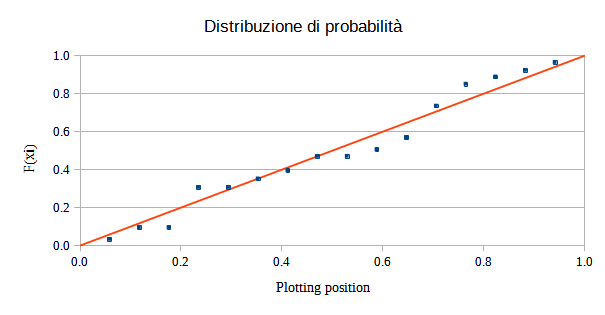
\includegraphics[scale=0.75]{immagini/distr_prob_15min.png}
\end{figure}

\subsection{Tempo di pioggia di 30 minuti}

\begin{table}[H]
    \caption*{Evento pluviometrico di 30 minuti.}
    \begin{minipage}{.5\linewidth}
      \caption{\textcolor{red}{Campione della serie pluviometrica.}}
      \centering
        \begin{tabular}{cccc}
            \toprule
            & dd-mm-yy   & hh:mm:ss & mm \\
            \midrule
         1  & 29/08/2020 & 17:45:00 & 39.8 \\
         2  & 05/09/2008 & 03:15:00 & 36.2 \\
         3  & 09/08/2015 & 13:00:00 & 33.2 \\
         4  & 10/08/2006 & 15:45:00 & 31.4 \\
         5  & 20/10/2013 & 19:30:00 & 30.6 \\
         6  & 03/08/2006 & 16:15:00 & 27   \\
         7  & 29/06/2014 & 19:45:00 & 27   \\
         8  & 15/06/2020 & 12:15:00 & 27   \\
         9  & 26/09/2021 & 11:00:00 & 27   \\
         10 & 15/09/2022 & 13:45:00 & 26.4 \\
         11 & 24/09/2012 & 14:30:00 & 26.2 \\
         12 & 28/10/2018 & 12:15:00 & 25.8 \\
         13 & 15/10/2019 & 15:15:00 & 25.4 \\
         14 & 15/09/2014 & 16:15:00 & 25.2 \\
         15 & 16/09/2021 & 07:45:00 & 25   \\
         16 & 16/09/2021 & 17:15:00 & 24.8 \\
         17 & 03/08/2020 & 14:00:00 & 24   \\
         18 & 25/07/2012 & 12:45:00 & 23.6 \\
         \bottomrule
        \end{tabular}
    \end{minipage}%
    \begin{minipage}{.5\linewidth}
      \centering
        \caption{\textcolor{red}{Parametri della serie pluviometrica.}}
        \begin{tabular}{cc}
            \toprule
        n        &     18    \\
        N        & 17 anni \\
        soglia   &    23.5     \\
        $\bar{x}$ &  28.0889      \\
        $\sigma$ &    4.4427     \\
        $\xi$      &  -0.0334     \\
        $\psi$      &  4.7424   \\
        $\lambda$   &  1.0588  \\
    \bottomrule     
        \end{tabular}
    \end{minipage} 
\end{table}

\begin{table}[H] \centering
    \caption{\textcolor{red}{Valori di distribuzione della serie di precipitazione della durata di 30 min.}}
            \begin{tabular}{cccc}
                \toprule
               & mm   & Plotting & F(xi)  \\
            \midrule
            1  & 23.6 & 0.0526   & 0.0209 \\
            2  & 24   & 0.1053   & 0.1002 \\
            3  & 24.8 & 0.1579   & 0.2407 \\
            4  & 25   & 0.2105   & 0.2724 \\
            5  & 25.2 & 0.2632   & 0.3028 \\
            6  & 25.4 & 0.3158   & 0.3319 \\
            7  & 25.8 & 0.3684   & 0.3867 \\
            8  & 26.2 & 0.4211   & 0.4372 \\
            9  & 26.4 & 0.4737   & 0.4609 \\
            10 & 27   & 0.5263   & 0.5264 \\
            11 & 27   & 0.5789   & 0.5264 \\
            12 & 27   & 0.6316   & 0.5264 \\
            13 & 27   & 0.6842   & 0.5264 \\
            14 & 30.6 & 0.7368   & 0.7847 \\
            15 & 31.4 & 0.7895   & 0.8199 \\
            16 & 33.2 & 0.8421   & 0.8798 \\
            17 & 36.2 & 0.8947   & 0.9395 \\
            18 & 39.8 & 0.9474   & 0.9740 \\
            \bottomrule
            \end{tabular}
\end{table}

\begin{figure}[H]\centering
    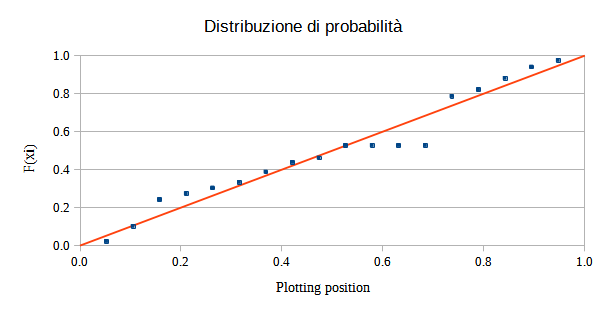
\includegraphics[scale=0.75]{immagini/distr_prob_30min.png}
\end{figure}

\subsection{Tempo di pioggia di 45 minuti}

\begin{table}[H]
    \caption*{Evento pluviometrico di 45 minuti.}
    \begin{minipage}{.5\linewidth}
      \caption{\textcolor{red}{Campione della serie pluviometrica.}}
      \centering
        \begin{tabular}{cccc}
            \toprule
            & dd-mm-yy   & hh:mm:ss & mm \\
         \midrule
         1  & 20/10/2013 & 19:45:00 & 48   \\
         2  & 29/08/2020 & 17:45:00 & 46.6 \\
         3  & 05/09/2008 & 03:30:00 & 37.2 \\
         4  & 29/06/2014 & 20:00:00 & 35.8 \\
         5  & 16/09/2021 & 17:15:00 & 35.8 \\
         6  & 26/09/2021 & 11:15:00 & 35   \\
         7  & 10/08/2006 & 16:00:00 & 34.8 \\
         8  & 09/08/2015 & 13:15:00 & 34.8 \\
         9  & 15/09/2022 & 13:45:00 & 33.2 \\
         10 & 28/10/2018 & 12:15:00 & 32.2 \\
         11 & 03/08/2006 & 16:30:00 & 32   \\
         12 & 10/11/2012 & 22:15:00 & 30.8 \\
         13 & 15/10/2019 & 15:15:00 & 30.4 \\
         14 & 17/09/2018 & 15:00:00 & 29.4 \\
         15 & 24/09/2012 & 14:30:00 & 28.6 \\
         16 & 15/06/2020 & 12:30:00 & 27.8 \\
         17 & 26/08/2012 & 04:30:00 & 27   \\
         18 & 25/07/2012 & 13:00:00 & 26.8 \\
         \bottomrule
        \end{tabular}
    \end{minipage}%
    \begin{minipage}{.5\linewidth}
      \centering
        \caption{\textcolor{red}{Parametri della serie pluviometrica.}}
        \begin{tabular}{cc}
            \toprule
            n        &    18     \\
            N        & 17 anni \\
            soglia   &      26.7   \\
            $\bar{x}$ &    33.6778    \\
            $\sigma$ &     5.9040    \\
            $\xi$      &   -0.1984    \\
            $\psi$      &   8.3623  \\
            $\lambda$   &  1.0588  \\
        \bottomrule     
        \end{tabular}
    \end{minipage} 
\end{table}

\begin{table}[H] \centering
    \caption{\textcolor{red}{Valori di distribuzione della serie di precipitazione della durata di 45 min.}}
            \begin{tabular}{cccc}
            \toprule
               & mm   & plotting & F(xi)  \\
            \midrule
            1  & 26.8 & 0.0526   & 0.0119 \\
            2  & 27   & 0.1053   & 0.0354 \\
            3  & 27.8 & 0.1579   & 0.1248 \\
            4  & 28.6 & 0.2105   & 0.2074 \\
            5  & 29.4 & 0.2632   & 0.2837 \\
            6  & 30.4 & 0.3158   & 0.3707 \\
            7  & 30.8 & 0.3684   & 0.4030 \\
            8  & 32   & 0.4211   & 0.4920 \\
            9  & 32.2 & 0.4737   & 0.5058 \\
            10 & 33.2 & 0.5263   & 0.5701 \\
            11 & 34.8 & 0.5789   & 0.6589 \\
            12 & 34.8 & 0.6316   & 0.6589 \\
            13 & 35   & 0.6842   & 0.6689 \\
            14 & 35.8 & 0.7368   & 0.7065 \\
            15 & 35.8 & 0.7895   & 0.7065 \\
            16 & 37.2 & 0.8421   & 0.7640 \\
            17 & 46.6 & 0.8947   & 0.9601 \\
            18 & 48   & 0.9474   & 0.9712 \\
            \bottomrule
            \end{tabular}
\end{table}

\begin{figure}[H]\centering
    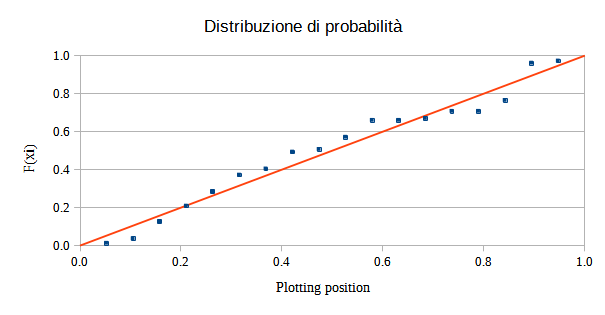
\includegraphics[scale=0.75]{immagini/distr_prob_45min.png}
\end{figure}

\subsection{Tempo di pioggia di 60 minuti}

\begin{table}[H]
    \caption*{Evento pluviometrico di 60 minuti.}
    \begin{minipage}{.5\linewidth}
      \caption{\textcolor{red}{Campione della serie pluviometrica.}}
      \centering
        \begin{tabular}{cccc}
            \toprule
            & dd-mm-yy   & hh:mm:ss & mm \\
         \midrule
         1  & 20/10/2013 & 19:45:00 & 59.4 \\
         2  & 29/08/2020 & 17:45:00 & 56.6 \\
         3  & 16/09/2021 & 17:15:00 & 49.4 \\
         4  & 29/06/2014 & 20:00:00 & 44.4 \\
         5  & 05/09/2008 & 03:45:00 & 44   \\
         6  & 26/09/2021 & 11:30:00 & 39.4 \\
         7  & 03/08/2006 & 16:45:00 & 38.4 \\
         8  & 28/10/2018 & 12:30:00 & 38   \\
         9  & 10/11/2012 & 22:15:00 & 37.8 \\
         10 & 15/09/2022 & 13:45:00 & 37.8 \\
         11 & 10/08/2006 & 16:15:00 & 36   \\
         12 & 09/08/2015 & 13:30:00 & 35.6 \\
         13 & 03/08/2020 & 14:30:00 & 35.6 \\
         14 & 16/09/2021 & 08:15:00 & 33.8 \\
         15 & 26/08/2012 & 04:45:00 & 33.4 \\
         16 & 15/10/2019 & 15:30:00 & 32.8 \\
         \bottomrule
        \end{tabular}
    \end{minipage}%
    \begin{minipage}{.5\linewidth}
      \centering
        \caption{\textcolor{red}{Parametri della serie pluviometrica.}}
        \begin{tabular}{cc}
            \toprule
            n        &    16     \\
            N        & 17 anni \\
            soglia   &      32.7   \\
            $\bar{x}$ &    40.7750    \\
            $\sigma$ &     8.0465    \\
            $\xi$      &   -0.0035    \\
            $\psi$      &   8.1037  \\
            $\lambda$   &   0.9412 \\
        \bottomrule     
        \end{tabular}
    \end{minipage} 
\end{table}

\begin{table}[H] \centering
    \caption{\textcolor{red}{Valori di distribuzione della serie di precipitazione della durata di 60 min.}}
            \begin{tabular}{cccc}
            \toprule
               & mm   & plotting & F(xi)  \\
            \midrule
            1  & 32.8 & 0.0588   & 0.0123 \\
            2  & 33.4 & 0.1176   & 0.0828 \\
            3  & 33.8 & 0.1765   & 0.1270 \\
            4  & 35.6 & 0.2353   & 0.3010 \\
            5  & 35.6 & 0.2941   & 0.3010 \\
            6  & 36   & 0.3529   & 0.3347 \\
            7  & 37.8 & 0.4118   & 0.4674 \\
            8  & 37.8 & 0.4706   & 0.4674 \\
            9  & 38   & 0.5294   & 0.4804 \\
            10 & 38.4 & 0.5882   & 0.5055 \\
            11 & 39.4 & 0.6471   & 0.5631 \\
            12 & 44   & 0.7059   & 0.7529 \\
            13 & 44.4 & 0.7647   & 0.7648 \\
            14 & 49.4 & 0.8235   & 0.8736 \\
            15 & 56.6 & 0.8824   & 0.9484 \\
            16 & 59.4 & 0.9412   & 0.9636 \\
            \bottomrule
            \end{tabular}
\end{table}

\begin{figure}[H]\centering
    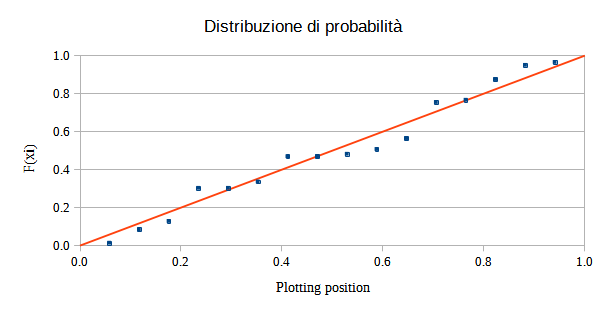
\includegraphics[scale=0.75]{immagini/distr_prob_60min.png}
\end{figure}

\subsection{Tempo di pioggia di 120 minuti}

\begin{table}[H]
    \caption*{Evento pluviometrico di 120 minuti.}
    \begin{minipage}{.5\linewidth}
      \caption{\textcolor{red}{Campione della serie pluviometrica.}}
      \centering
        \begin{tabular}{cccc}
            \toprule
            & dd-mm-yy   & hh:mm:ss & mm \\
         \midrule
         1  & 20/10/2013 & 20:30:00 & 68.6 \\
         2  & 29/08/2020 & 18:00:00 & 67.8 \\
         3  & 16/09/2021 & 17:30:00 & 64.8 \\
         4  & 28/10/2018 & 12:30:00 & 58.8 \\
         5  & 10/11/2012 & 22:30:00 & 56.2 \\
         6  & 03/08/2006 & 17:45:00 & 54.8 \\
         7  & 05/09/2008 & 03:15:00 & 51.8 \\
         8  & 26/08/2012 & 05:30:00 & 51.8 \\
         9  & 05/11/2014 & 07:00:00 & 51.2 \\
         10 & 26/09/2021 & 11:30:00 & 50.6 \\
         11 & 15/09/2022 & 13:45:00 & 49.8 \\
         12 & 03/08/2020 & 14:30:00 & 49.2 \\
         13 & 29/06/2014 & 20:15:00 & 47   \\
         14 & 11/12/2017 & 23:45:00 & 41.8 \\
         15 & 20/09/2014 & 04:15:00 & 40.8 \\
         16 & 25/06/2014 & 09:15:00 & 40.4 \\
         17 & 09/02/2016 & 21:15:00 & 40   \\
         \bottomrule  
        \end{tabular}
    \end{minipage}%
    \begin{minipage}{.5\linewidth}
      \centering
        \caption{\textcolor{red}{Parametri della serie pluviometrica.}}
        \begin{tabular}{cc}
            \toprule
            n        &     17    \\
            N        & 17 anni \\
            soglia   &     39.9    \\
            $\bar{x}$ &   52.0824     \\
            $\sigma$ &     9.0452    \\
            $\xi$      &     -0.4070  \\
            $\psi$      &   17.1403  \\
            $\lambda$   &   1.0000 \\
        \bottomrule           
        \end{tabular}
    \end{minipage} 
\end{table}

\begin{table}[H] \centering
    \caption{\textcolor{red}{Valori di distribuzione della serie di precipitazione della durata di 120 min.}}
        \begin{tabular}{cccc}
            \toprule
           & mm   & plotting & F(xi)  \\
        \midrule
        1  & 40   & 0.0556   & 0.0058 \\
        2  & 40.4 & 0.1111   & 0.0289 \\
        3  & 40.8 & 0.1667   & 0.0517 \\
        4  & 41.8 & 0.2222   & 0.1072 \\
        5  & 47   & 0.2778   & 0.3647 \\
        6  & 49.2 & 0.3333   & 0.4583 \\
        7  & 49.8 & 0.3889   & 0.4823 \\
        8  & 50.6 & 0.4444   & 0.5134 \\
        9  & 51.2 & 0.5000   & 0.5359 \\
        10 & 51.8 & 0.5556   & 0.5578 \\
        11 & 51.8 & 0.6111   & 0.5578 \\
        12 & 54.8 & 0.6667   & 0.6580 \\
        13 & 56.2 & 0.7222   & 0.6996 \\
        14 & 58.8 & 0.7778   & 0.7686 \\
        15 & 64.8 & 0.8333   & 0.8890 \\
        16 & 67.8 & 0.8889   & 0.9307 \\
        17 & 68.6 & 0.9444   & 0.9398 \\
        \bottomrule
        \end{tabular}
\end{table}

\begin{figure}[H]\centering
    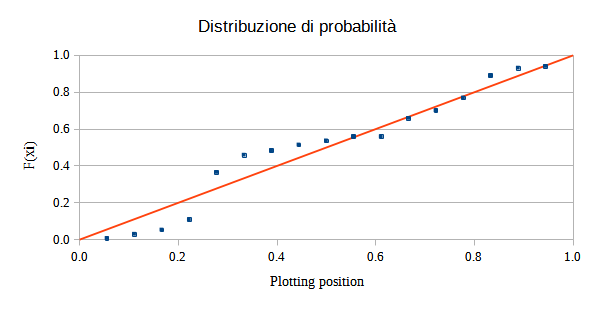
\includegraphics[scale=0.75]{immagini/distr_prob_120.png}
\end{figure}

\subsection{Tempo di pioggia di 180 minuti}

\begin{table}[H]
    \caption*{Evento pluviometrico di 180 minuti.}
    \begin{minipage}{.5\linewidth}
      \caption{\textcolor{red}{Campione della serie pluviometrica.}}
      \centering
        \begin{tabular}{cccc}
            \toprule
            & dd-mm-yy   & hh:mm:ss & mm \\
         \midrule
         1  & 16/09/2021 & 18:15:00 & 73.8 \\
         2  & 29/08/2020 & 19:15:00 & 73   \\
         3  & 20/10/2013 & 20:45:00 & 72.6 \\
         4  & 28/10/2018 & 12:15:00 & 72.4 \\
         5  & 03/08/2020 & 14:30:00 & 67.8 \\
         6  & 05/11/2014 & 07:00:00 & 67.4 \\
         7  & 10/11/2012 & 23:00:00 & 65.4 \\
         8  & 03/08/2006 & 18:45:00 & 62.6 \\
         9  & 26/09/2021 & 12:30:00 & 61.8 \\
         10 & 15/09/2022 & 13:45:00 & 61   \\
         11 & 05/09/2008 & 04:00:00 & 60.4 \\
         12 & 20/09/2014 & 04:15:00 & 59.4 \\
         13 & 12/12/2017 & 01:00:00 & 59.4 \\
         14 & 09/02/2016 & 21:45:00 & 57.4 \\
         15 & 20/01/2009 & 10:00:00 & 55   \\
         16 & 26/08/2012 & 06:30:00 & 54.4 \\
         \bottomrule
        \end{tabular}
    \end{minipage}%
    \begin{minipage}{.5\linewidth}
      \centering
        \caption{\textcolor{red}{Parametri della serie pluviometrica.}}
        \begin{tabular}{cc}
            \toprule
            n        &    16     \\
            N        & 17 anni \\
            soglia   &     54.3    \\
            $\bar{x}$ &  63.9875\\
            $\sigma$ &   6.5183  \\
            $\xi$    &    -0.6044  \\
            $\psi$      &    15.5427 \\
            $\lambda$   &    0.9412\\
        \bottomrule     
        \end{tabular}
    \end{minipage} 
\end{table}

\begin{table}[H] \centering
    \caption{\textcolor{red}{Valori di distribuzione della serie di precipitazione della durata di 180 min.}}
            \begin{tabular}{cccc}
            \toprule
               & mm   & plotting & F(xi)  \\
            \midrule
            1  & 54.4 & 0.0588   & 0.0064 \\
            2  & 55   & 0.1176   & 0.0446 \\
            3  & 57.4 & 0.1765   & 0.1915 \\
            4  & 59.4 & 0.2353   & 0.3063 \\
            5  & 59.4 & 0.2941   & 0.3063 \\
            6  & 60.4 & 0.3529   & 0.3611 \\
            7  & 61   & 0.4118   & 0.3931 \\
            8  & 61.8 & 0.4706   & 0.4348 \\
            9  & 62.6 & 0.5294   & 0.4752 \\
            10 & 65.4 & 0.5882   & 0.6073 \\
            11 & 67.4 & 0.6471   & 0.6922 \\
            12 & 67.8 & 0.7059   & 0.7082 \\
            13 & 72.4 & 0.7647   & 0.8665 \\
            14 & 72.6 & 0.8235   & 0.8722 \\
            15 & 73   & 0.8824   & 0.8834 \\
            16 & 73.8 & 0.9412   & 0.9046 \\
            \bottomrule
            \end{tabular}
\end{table}

\begin{figure}[H]\centering
    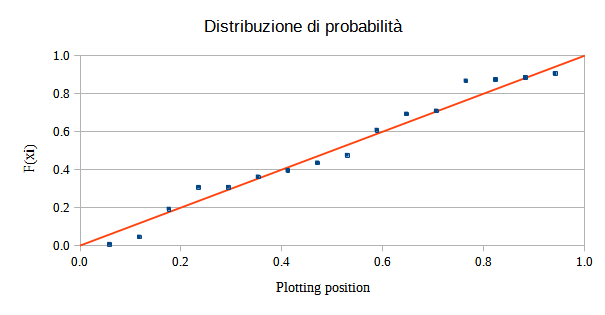
\includegraphics[scale=0.75]{immagini/distr_prob_180min.png}
\end{figure}

\subsection{Tempo di pioggia di 360 minuti}

\begin{table}[H]
    \caption*{Evento pluviometrico di 360 minuti.}
    \begin{minipage}{.5\linewidth}
      \caption{\textcolor{red}{Campione della serie pluviometrica.}}
      \centering
        \begin{tabular}{cccc}
            \toprule
            & dd-mm-yy   & hh:mm:ss & mm  \\
         \midrule
         1  & 05/11/2014 & 07:45:00 & 119.6 \\
         2  & 16/09/2021 & 18:30:00 & 116.8 \\
         3  & 20/01/2009 & 12:45:00 & 103.2 \\
         4  & 11/11/2012 & 02:45:00 & 100.4 \\
         5  & 01/02/2019 & 21:30:00 & 97    \\
         6  & 09/02/2016 & 22:15:00 & 96.2  \\
         7  & 12/12/2017 & 00:15:00 & 95.2  \\
         8  & 28/10/2018 & 14:30:00 & 88.2  \\
         9  & 26/09/2021 & 15:30:00 & 85.8  \\
         10 & 23/12/2009 & 02:15:00 & 85.4  \\
         11 & 05/12/2008 & 06:15:00 & 84.6  \\
         12 & 18/03/2013 & 12:30:00 & 81.2  \\
         13 & 15/09/2022 & 15:15:00 & 79.6  \\
         14 & 10/12/2017 & 23:45:00 & 79    \\
         15 & 05/03/2006 & 11:00:00 & 78.4  \\
         16 & 04/01/2014 & 18:15:00 & 77.8  \\
         17 & 29/08/2020 & 19:45:00 & 77.6  \\
         18 & 20/10/2013 & 21:15:00 & 76.8  \\
         19 & 02/03/2020 & 17:30:00 & 76    \\
         \bottomrule
        \end{tabular}
    \end{minipage}%
    \begin{minipage}{.5\linewidth}
      \centering
        \caption{\textcolor{red}{Parametri della serie pluviometrica.}}
        \begin{tabular}{ll}
            \toprule
            n        &   19      \\
            N        & 17 anni \\
            soglia   &   75.9      \\
            $\bar{x}$ &    89.4105    \\
            $\sigma$ &     13.2704    \\
            $\xi$      &     -0.0183  \\
            $\psi$      &  13.7572   \\
            $\lambda$   &   1.1176 \\
        \bottomrule        
        \end{tabular}
    \end{minipage} 
\end{table}

\begin{table}[H] \centering
    \caption{\textcolor{red}{Valori di distribuzione della serie di precipitazione della durata di 360 min.}}
            \begin{tabular}{cccc}
            \toprule
               & mm    & plotting & F(xi)  \\
            \midrule
            1  & 76    & 0.0500   & 0.0072 \\
            2  & 76.8  & 0.1000   & 0.0634 \\
            3  & 77.6  & 0.1500   & 0.1164 \\
            4  & 77.8  & 0.2000   & 0.1291 \\
            5  & 78.4  & 0.2500   & 0.1664 \\
            6  & 79    & 0.3000   & 0.2021 \\
            7  & 79.6  & 0.3500   & 0.2363 \\
            8  & 81.2  & 0.4000   & 0.3206 \\
            9  & 84.6  & 0.4500   & 0.4706 \\
            10 & 85.4  & 0.5000   & 0.5009 \\
            11 & 85.8  & 0.5500   & 0.5154 \\
            12 & 88.2  & 0.6000   & 0.5940 \\
            13 & 95.2  & 0.6500   & 0.7586 \\
            14 & 96.2  & 0.7000   & 0.7759 \\
            15 & 97    & 0.7500   & 0.7889 \\
            16 & 100.4 & 0.8000   & 0.8364 \\
            17 & 103.2 & 0.8500   & 0.8675 \\
            18 & 116.8 & 0.9000   & 0.9530 \\
            19 & 119.6 & 0.9500   & 0.9621 \\
            \bottomrule
            \end{tabular}
\end{table}

\begin{figure}[H]\centering
    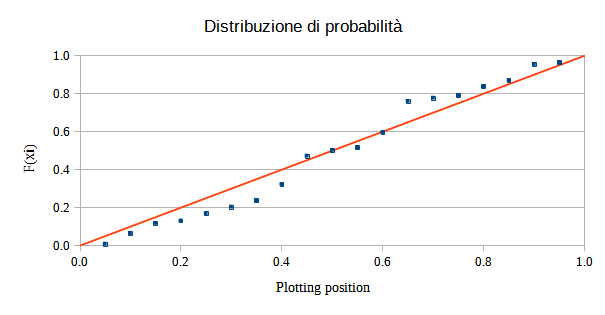
\includegraphics[scale=0.75]{immagini/distr_prob_360min.png}
\end{figure}

\subsection{Tempo di pioggia di 720 minuti}

\begin{table}[H]
    \caption*{Evento pluviometrico di 720 minuti.}
    \begin{minipage}{.5\linewidth}
      \caption{\textcolor{red}{Campione della serie pluviometrica.}}
      \centering
        \begin{tabular}{cccc}
            \toprule
            & dd-mm-yy   & hh:mm:ss & mm  \\
         \midrule
         1  & 12/12/2017 & 01:30:00 & 183   \\
         2  & 02/02/2019 & 01:45:00 & 173.2 \\
         3  & 20/01/2009 & 13:30:00 & 173   \\
         4  & 16/09/2021 & 17:45:00 & 167.2 \\
         5  & 05/12/2008 & 11:15:00 & 161.6 \\
         6  & 05/11/2014 & 12:45:00 & 151   \\
         7  & 11/11/2012 & 07:15:00 & 148   \\
         8  & 28/10/2018 & 13:15:00 & 146.2 \\
         9  & 25/12/2009 & 01:15:00 & 137.8 \\
         10 & 21/12/2019 & 00:30:00 & 124.7 \\
         11 & 04/01/2014 & 22:30:00 & 121.8 \\
         12 & 23/12/2009 & 02:45:00 & 119.4 \\
         13 & 10/02/2016 & 01:30:00 & 113   \\
         14 & 08/12/2017 & 14:15:00 & 111.8 \\
         15 & 11/01/2016 & 13:45:00 & 109.2 \\
         16 & 18/03/2013 & 16:45:00 & 106.2 \\
         17 & 25/10/2011 & 23:00:00 & 105   \\
         \bottomrule
        \end{tabular}
    \end{minipage}%
    \begin{minipage}{.5\linewidth}
      \centering
        \caption{\textcolor{red}{Parametri della serie pluviometrica.}}
        \begin{tabular}{cc}
            \toprule
            n        &   17      \\
            N        & 17 anni \\
            soglia   &     104.9    \\
            $\bar{x}$ &    138.3588    \\
            $\sigma$ &      26.5273   \\
            $\xi$      &     -0.2954  \\
            $\psi$      &    43.3438 \\
            $\lambda$   &   1.0000 \\
        \bottomrule     
        \end{tabular}
    \end{minipage} 
\end{table}

\begin{table}[H] \centering
    \caption{\textcolor{red}{Valori di distribuzione della serie di precipitazione della durata di 720 min.}}
            \begin{tabular}{cccc} 
            \toprule
               & mm    & plotting & F(xi)  \\
            \midrule
            1  & 105   & 0.0556   & 0.0023 \\
            2  & 106.2 & 0.1111   & 0.0297 \\
            3  & 109.2 & 0.1667   & 0.0958 \\
            4  & 111.8 & 0.2222   & 0.1505 \\
            5  & 113   & 0.2778   & 0.1749 \\
            6  & 119.4 & 0.3333   & 0.2969 \\
            7  & 121.8 & 0.3889   & 0.3392 \\
            8  & 124.7 & 0.4444   & 0.3878 \\
            9  & 137.8 & 0.5000   & 0.5766 \\
            10 & 146.2 & 0.5556   & 0.6734 \\
            11 & 148   & 0.6111   & 0.6919 \\
            12 & 151   & 0.6667   & 0.7211 \\
            13 & 161.6 & 0.7222   & 0.8086 \\
            14 & 167.2 & 0.7778   & 0.8460 \\
            15 & 173   & 0.8333   & 0.8790 \\
            16 & 173.2 & 0.8889   & 0.8800 \\
            17 & 183   & 0.9444   & 0.9237 \\
            \bottomrule
            \end{tabular}
            \end{table}

\begin{figure}[H]\centering
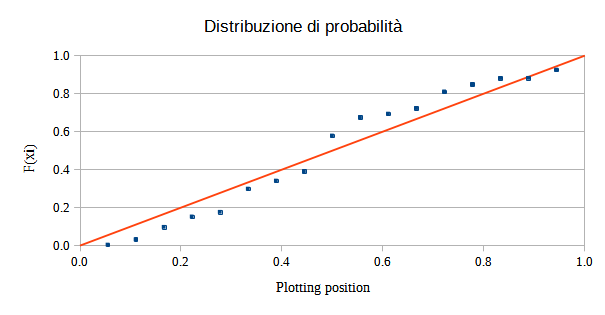
\includegraphics[scale=0.75]{immagini/distr_prob_720min.png}
\end{figure}

\subsection{Tempo di pioggia di 1440 minuti}

\begin{table}[H]
    \caption*{Evento pluviometrico di 1440 minuti.}
    \begin{minipage}{.5\linewidth}
      \caption{\textcolor{red}{Campione della serie pluviometrica.}}
      \centering
        \begin{tabular}{cccc}
            \toprule
            & dd-mm-yy   & hh:mm:ss & mm  \\
         \midrule
         1  & 12/12/2017 & 01:00:00 & 311.2 \\
         2  & 20/01/2009 & 15:15:00 & 250.4 \\
         3  & 02/02/2019 & 06:45:00 & 246.4 \\
         4  & 05/12/2008 & 17:00:00 & 220.4 \\
         5  & 21/12/2019 & 10:00:00 & 214.7 \\
         6  & 06/11/2014 & 00:15:00 & 200.8 \\
         7  & 17/09/2021 & 04:00:00 & 190.2 \\
         8  & 25/12/2009 & 10:15:00 & 179.2 \\
         9  & 11/11/2012 & 13:15:00 & 170.4 \\
         10 & 05/01/2014 & 08:00:00 & 167.8 \\
         11 & 23/12/2009 & 02:45:00 & 165   \\
         12 & 08/12/2017 & 19:30:00 & 163.6 \\
         13 & 22/01/2021 & 23:00:00 & 163   \\
         14 & 28/10/2018 & 16:45:00 & 155.2 \\
         15 & 05/12/2020 & 13:00:00 & 149.6 \\
         16 & 17/01/2014 & 22:30:00 & 143.6 \\
         \bottomrule
        \end{tabular}
    \end{minipage}%
    \begin{minipage}{.5\linewidth}
      \centering
        \caption{\textcolor{red}{Parametri della serie pluviometrica.}}
        \begin{tabular}{ll}
            \toprule
            n        &   16      \\
            N        & 17 anni \\
            soglia   &     143.5    \\
            $\bar{x}$ &    193.2188\\
            $\sigma$ &     45.4932    \\
            $\xi$      &     -0.0972  \\
            $\psi$      &   54.5512  \\
            $\lambda$   &   0.9412 \\
        \bottomrule        
        \end{tabular}
    \end{minipage} 
\end{table}

\begin{table}[H] \centering
    \caption{\textcolor{red}{Valori di distribuzione della serie di precipitazione della durata di 1440 min.}}
            \begin{tabular}{cccc}
            \toprule
               & mm    & plotting & F(xi)  \\
            \midrule
            1  & 143.6 & 0.0588   & 0.0018 \\
            2  & 149.6 & 0.1176   & 0.1063 \\
            3  & 155.2 & 0.1765   & 0.1949 \\
            4  & 163.6 & 0.2353   & 0.3129 \\
            5  & 165   & 0.2941   & 0.3309 \\
            6  & 167.8 & 0.3529   & 0.3658 \\
            7  & 170.4 & 0.4118   & 0.3967 \\
            8  & 170.8 & 0.4706   & 0.4013 \\
            9  & 179.2 & 0.5294   & 0.4914 \\
            10 & 190.2 & 0.5882   & 0.5909 \\
            11 & 201   & 0.6471   & 0.6711 \\
            12 & 214.7 & 0.7059   & 0.7523 \\
            13 & 220.4 & 0.7647   & 0.7804 \\
            14 & 246.4 & 0.8235   & 0.8755 \\
            15 & 250.4 & 0.8824   & 0.8863 \\
            16 & 311.2 & 0.9412   & 0.9741 \\
            \bottomrule
            \end{tabular}
\end{table}

\begin{figure}[H]\centering
    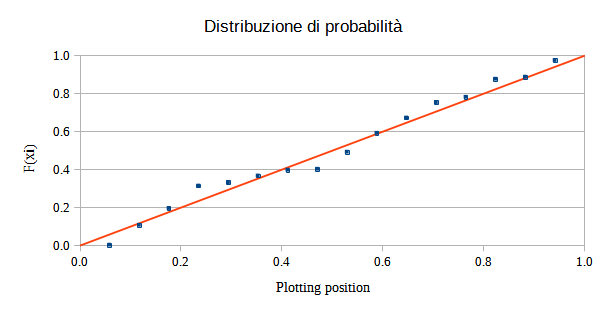
\includegraphics[scale=0.75]{immagini/distr_prob_1440min.png}
\end{figure}

\subsection{Altezze critiche e LSPP}

Successivamente ad aver valutato la bontà di accoppiamento degli eventi pluviometrici, è possibile calcolare l'altezza critica, dato un certo tempo di ritorno (215 anni per questo studio), mediante la formula \ref{h_critica_tr}.

\begin{table}[H] \centering
    \caption{\textcolor{red}{Altezze critiche di precipitazione, suddivise per durata di precipitazione.}}
            \begin{tabular}{ccc}
            \toprule
            Tempo di prec. [min] & Tempo di prec. [ore] & Altezza di pioggia [mm] \\
            \midrule
            15                       & 0.25                     & 29.91                       \\
            30                       & 0.5                      & 47.04                       \\
            45                       & 0.75                     & 54.49                       \\
            60                       & 1                        & 75.33                       \\
            120                      & 2                        & 77.28                       \\
            180                      & 3                        & 78.97                       \\
            360                      & 6                        & 147.66                      \\
            720                      & 12                       & 221.59                      \\
            1440                     & 24                       & 369.78                     \\
            \bottomrule
            \end{tabular}
\end{table}

\noindent Da questi dati è possibile creare un grafico che indichi l'andamento pluviometrico in funzione della durata dell'evento stesso.

\begin{figure}[H]\centering
    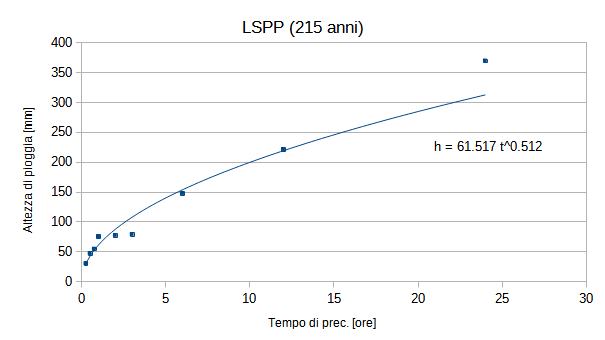
\includegraphics[scale=0.75]{immagini/LSPP_215.png}
    \caption{LSPP per un tempo di ritorno di 215 anni, con assi a scala lineare.}
\end{figure}

\begin{figure}[H]\centering
    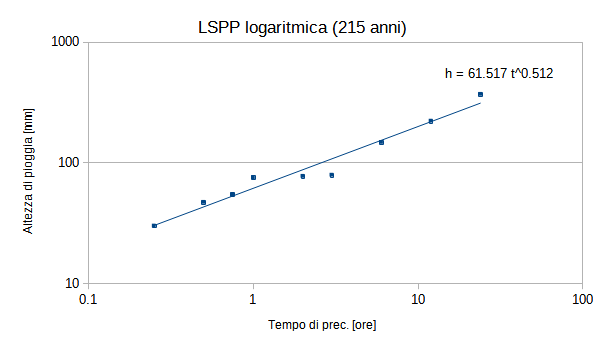
\includegraphics[scale=0.75]{immagini/LSPP_log_215.png}
    \caption{LSPP per un tempo di ritorno di 215 anni, con assi a scala logaritmica.}
\end{figure}

